\documentclass[11pt]{extarticle}

\usepackage[english,french]{babel}
\usepackage[utf8]{inputenc}
\usepackage{url}
\usepackage[T1]{fontenc}
\usepackage{booktabs}
\usepackage{enumitem}
\usepackage{graphicx}
\usepackage{pifont}
\usepackage{makecell}
\setcellgapes{1pt}
\usepackage{placeins}
\usepackage{subcaption}
\usepackage{pgfplots}
\usetikzlibrary{calc}
\pgfplotsset{compat=1.18}
\usepgfplotslibrary{dateplot}
\usepackage[margin=1in]{geometry}
\usepackage[colorlinks=true, allcolors=blue]{hyperref}
\usepackage{amsmath}
\usepackage{pgfplotstable}
\usepackage{amsfonts}
\usepgfplotslibrary{groupplots}

\usetikzlibrary{backgrounds}

\title{
    \hspace*{-12cm}
    \vspace*{1cm}
    \protect\\
    \vspace*{1cm}
    \textbf{Long Term Memory Processes Using Hurst Estimation}
}

\author{Remiat Alexandre}

\date{\today}

\graphicspath{{img/}}

\xdefinecolor{kblue}{RGB}{0,38,69}
\xdefinecolor{korange}{RGB}{255,128,89}
\xdefinecolor{kgray}{RGB}{47,108,130}
\xdefinecolor{kgreen}{RGB}{102,143,72}


\begin{document}

\selectlanguage{english}

\maketitle


\newpage


\section*{Abstract}

This paper presents a study on long-term memory processes in financial time series using Hurst estimation methods, specifically the traditional R/S statistic (Rescaled Range analysis) and the Modified R/S statistic.
The R/S statistic and the Modified R/S statistic are computed to determine the presence of long-range dependence in the time series data. The Hurst exponent, derived from both statistics, is used to characterize the memory behavior of the series.


\newpage

\section{Introduction}

The Hurst exponent is a key measure in the study of time series data, used primarily to analyze the long-term memory and self-similarity of stochastic processes. First introduced by the British hydrologist Harold Hurst in the 1950s to study river flow data, the Hurst exponent has since found widespread application in various fields, including finance, physics, and environmental science. The exponent provides insights into the persistence or mean-reversion behavior of a time series: a value greater than 0.5 indicates long-range dependence and persistence, while a value less than 0.5 suggests mean-reverting behavior.

The most commonly used method to estimate the Hurst exponent is the Rescaled Range (R/S) analysis, introduced by Hurst and later refined by Mandelbrot. However, the traditional R/S statistic has limitations, particularly in its sensitivity to short-term memory effects, which can obscure long-range dependence in the data. To address these issues, Lo (1991) proposed the Modified R/S statistic, which improves the estimation of the Hurst exponent by accounting for short-term autocorrelation.

This paper presents an analysis of time series data using both the traditional R/S statistic and the Modified R/S statistic, with a focus on their ability to detect long memory in financial data. We apply these methods to a range of stock market indices and examine the significance of the Hurst exponent in characterizing market dynamics. Additionally, we discuss the critical values for the Modified R/S test, based on Lo’s (1991) table, to help identify whether a series exhibits long memory behavior.

Through this analysis, we aim to highlight the advantages of the Modified R/S statistic in overcoming the limitations of the traditional R/S method, providing a more robust framework for studying time series with long memory. This is particularly valuable in the context of financial markets, where long memory and fractal-like behavior are often observed.



\section{Fractional Brownian Motion}

Fractional Brownian motion (fBm) is a generalization of standard Brownian motion that introduces dependence in increments,
making it suitable for modeling processes with memory effects. It is a continuous-time Gaussian process \( X_H(t) \) H corresponds
to the Hurst exponent and \( H \in [0, 1] \) with the following properties:

\begin{itemize}
    \item \( X_H(0) = 0 \).
    \item The increments \( X_H(t) - X_H(s) \) follow a normal distribution with mean zero and variance:
    \begin{equation}
        \mathbb{E} \left[ (X_H(t) - X_H(s))^2 \right] = \sigma^2|t - s|^{2H},
    \end{equation}
    where \( H \) is the Hurst exponent.
    \item The process exhibits self-similarity, meaning that for any scaling factor \( c \), \( c \in \mathbb{R}^+ \), the rescaled process satisfies:
    \begin{equation}
        X_H(ct) \overset{d}{=} c^H X_H(t).
    \end{equation}
    \item When \( H = 0.5 \), fBm reduces to classical Brownian motion.
    \item For \( H > 0.5 \), the process exhibits long-term positive autocorrelation, meaning that an increase in the past tends to be followed by further increases.
    \item For \( H < 0.5 \), the process has anti-persistent behavior, where an increase in the past is more likely to be followed by a decrease.
\end{itemize}

The covariance function of fBm is given by:

\begin{equation}
    C_H(t_1, t_2) = \frac{\sigma^2}{2} \left( t_1^{2H} + t_2^{2H} - |t_1 - t_2|^{2H} \right),
    \label{eq:fbm_covariance}
\end{equation}

which accounts for the dependence structure of the process. The Hurst exponent \( H \) plays a critical role in determining the smoothness and correlation properties of fBm:

\begin{itemize}
    \item \textbf{For small \( H \) values} (\( H < 0.5 \)), the process is highly erratic, with rapid changes and weak memory effects.
    \item \textbf{For large \( H \) values} (\( H > 0.5 \)), the trajectory becomes smoother, and the process exhibits long-range dependence.
\end{itemize}

Fractional Brownian motion is widely used in finance, telecommunications, and physics to model phenomena exhibiting memory effects and self-similarity, such as stock market fluctuations, internet traffic, and geological formations.


\subsection{Simulation of Fractional Brownian Motion}

To generate the fractional Brownian motion (fBm), we use a Cholesky decomposition-based approach. The covariance matrix of fBm is given by \eqref{eq:fbm_covariance}:

where \( H \) is the Hurst exponent, which determines the degree of long-term dependence in the process.

The steps of the simulation are as follows:
\begin{enumerate}
    \item Define a time grid of \( N \) points between \( 0 \) and \( T \).
    \item Compute the covariance matrix using the formula above.
    \item Apply Cholesky decomposition to obtain a lower triangular matrix \( L \).
    \item Generate a vector \( W \) of standard normal random variables.
    \item Obtain the fBm path by computing \( X = L W \).
\end{enumerate}

The params used for this simulation are N = 1000, T = 1, and Hurst exponents \( H = 0.2, 0.3, 0.5, 0.6, 0.8 \), the number
of lag for the autocorrelation is 40.

\begin{figure}[!ht]
    \centering
    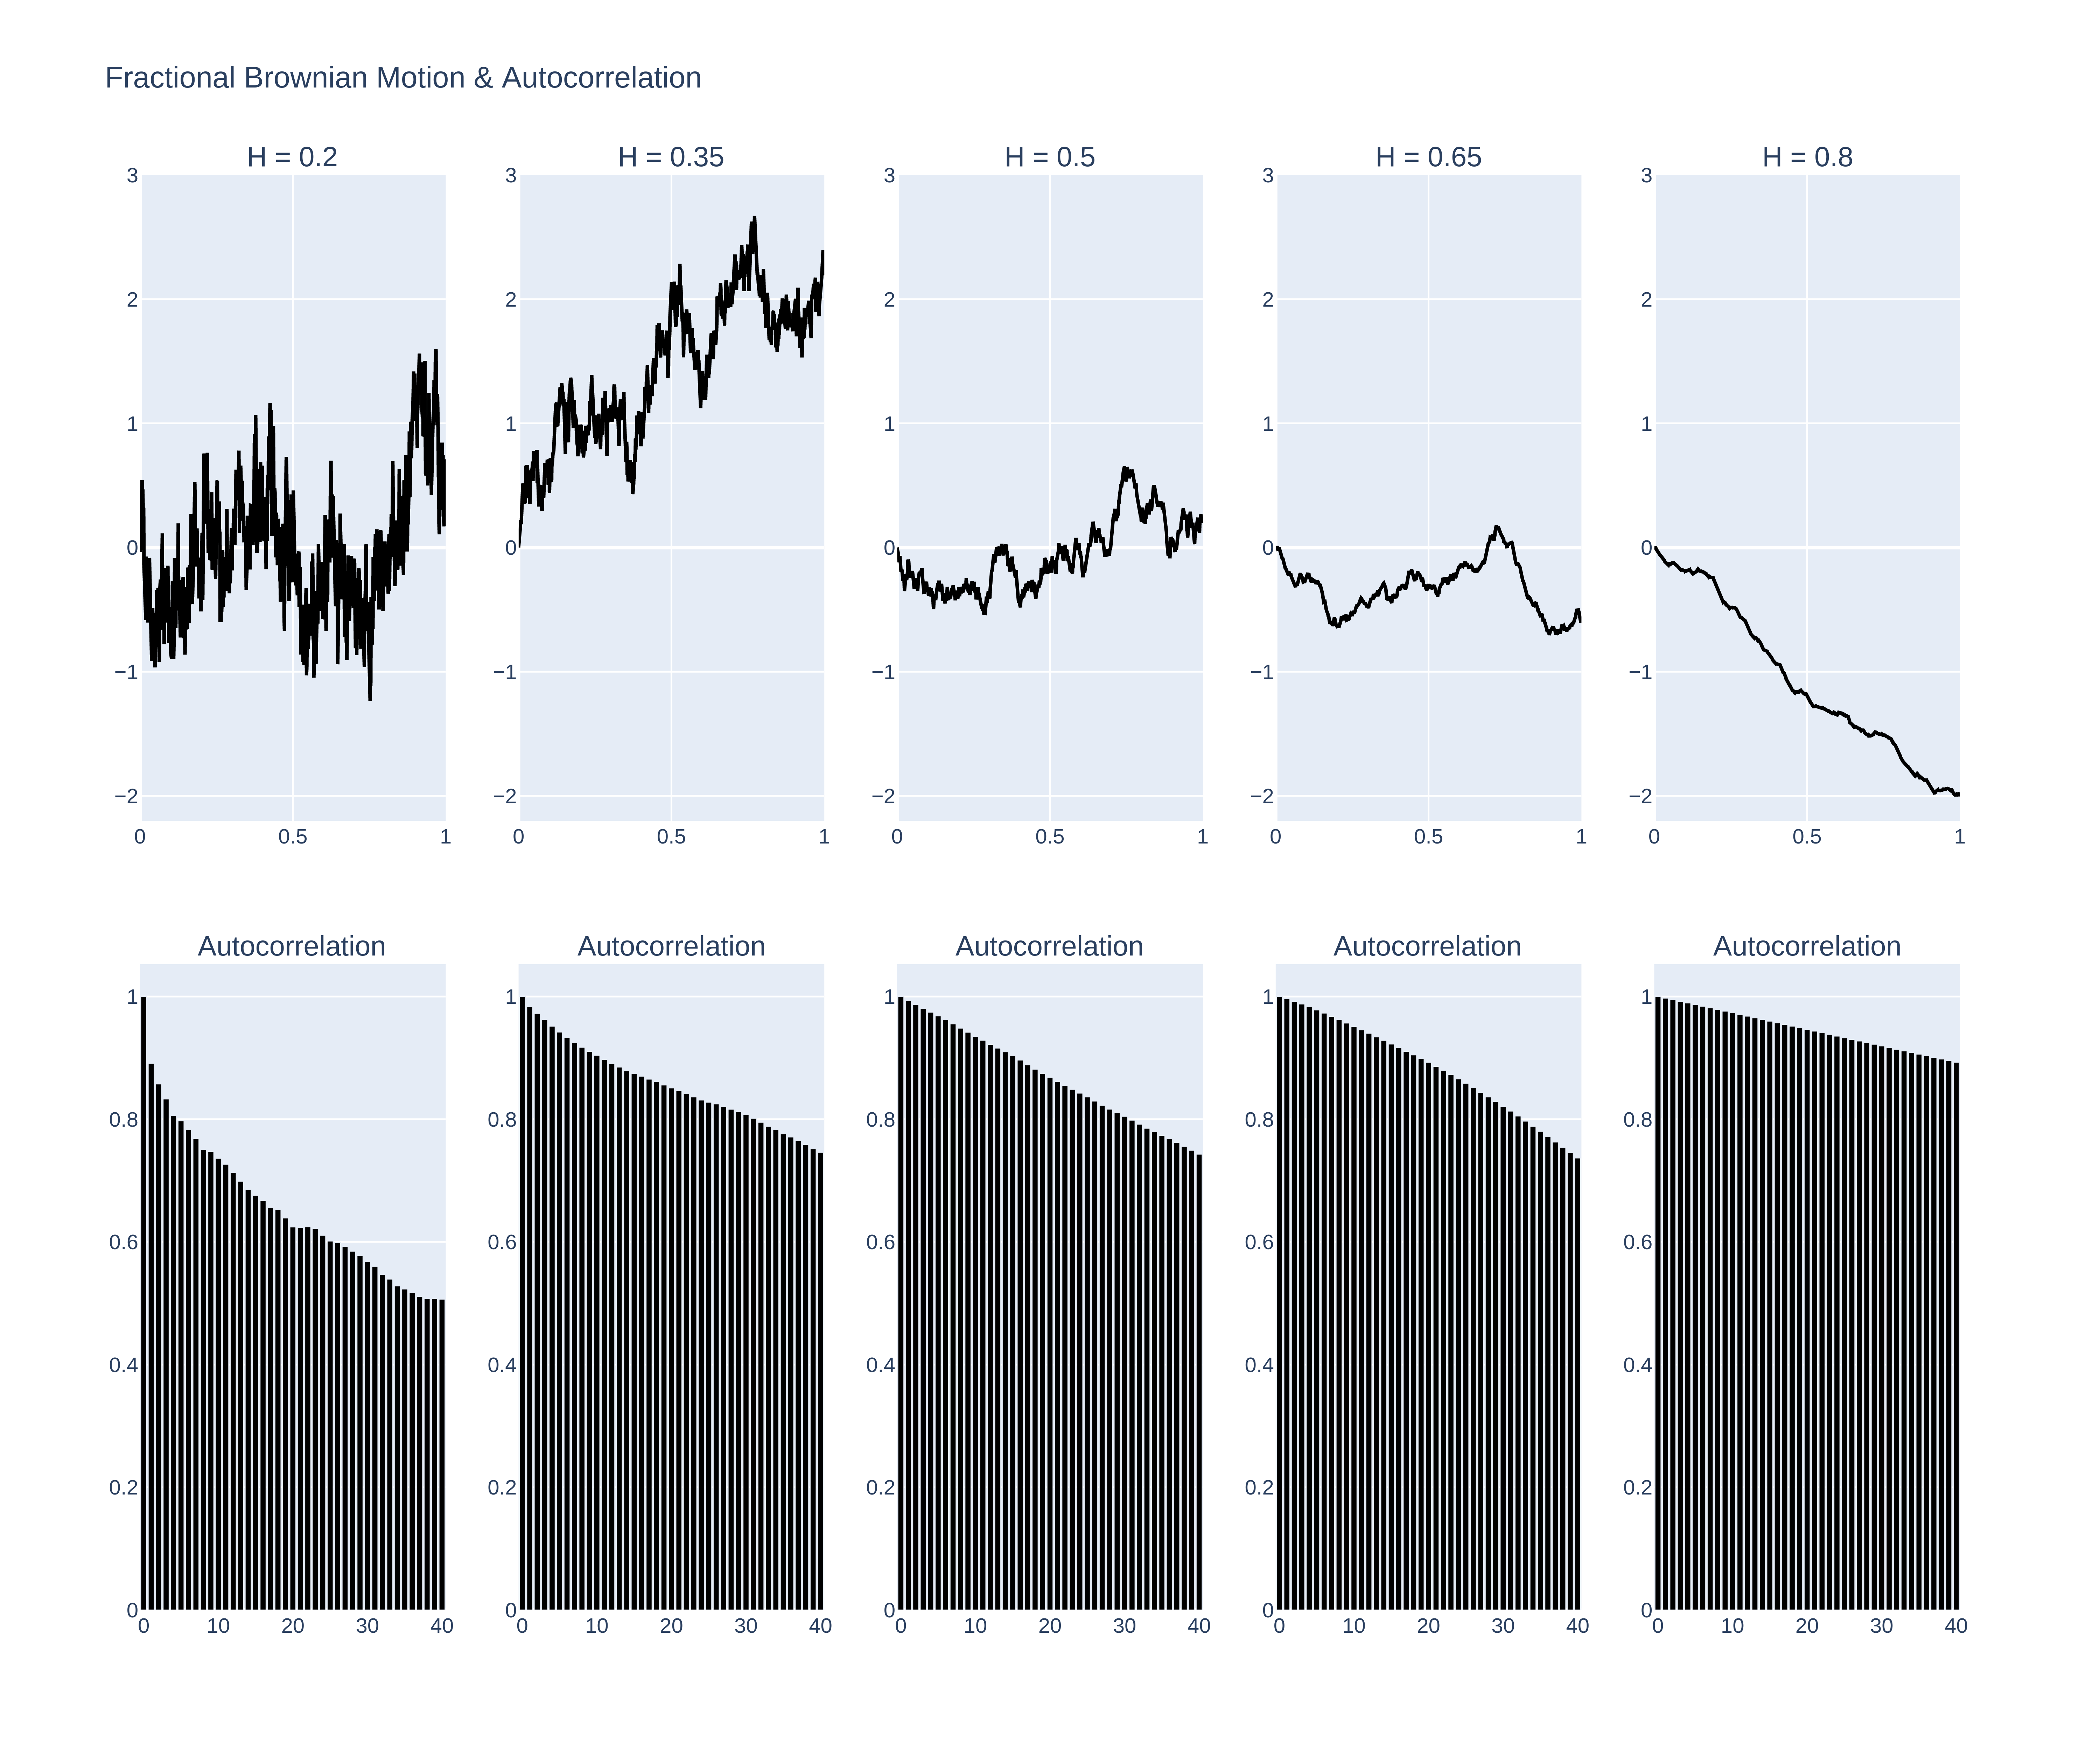
\includegraphics[width=0.8\textwidth]{img/fdm_autocorr}
    \caption{Simulation of Fractional Brownian Motion with different Hurst exponent and its autocorrelation function.}
    \label{fig:fbm_autocorr}
\end{figure}

\FloatBarrier

The behavior of the fractional Brownian motion (fBm) varies significantly with the Hurst exponent \( H \).

When \( H \) is small (close to 0), the fBm exhibits high local variability, resulting in a highly granular trajectory with frequent fluctuations. The autocorrelation of increments decays rapidly, indicating that future values are weakly influenced by past values. This suggests a short-memory process, similar to standard Brownian motion.

As \( H \) increases, the autocorrelation decays more slowly, meaning that past values have a more significant impact on future values. This introduces a form of long-term dependence, where the process exhibits persistent trends. Consequently, the fBm trajectory appears smoother, with larger coherent movements and fewer abrupt changes.

In summary, a lower \( H \) leads to a more irregular and noisy path, characteristic of short-memory processes, while a higher \( H \) results in a smoother trajectory with stronger persistence.

\subsection{Hurst Exponent Calculation}
\subsection{R/S and Modified R/S Analysis}
The R/S (Rescaled Range) analysis, introduced by Hurst and developed in various works by Mandelbrot, is certainly the most well-known method for estimating the Hurst exponent $H$. This statistic is defined as the range of the partial sums of deviations from the mean of a time series divided by its standard deviation. Consider a time series $Y_t$, $t = 1, ..., T$, with mean $\bar{Y}$. The range $R$ is defined as:

\[
R = \max_{1 \leq j \leq T} \left( Y_j - \bar{Y} \right) - \min_{1 \leq j \leq T} \left( Y_j - \bar{Y} \right)
\]

The R/S statistic is then computed by dividing the range by the standard deviation $s_T$ of the series:

\[
Q_T = \frac{R}{s_T} = \frac{\max_{1 \leq j \leq T} \left( Y_j - \bar{Y} \right) - \min_{1 \leq j \leq T} \left( Y_j - \bar{Y} \right)}{s_T}
\]

The R/S statistic, $Q_T$, is always positive. In various papers, Mandelbrot and Wallis (1969e), Mandelbrot (1973), and Mandelbrot and Taqqu (1979) have emphasized the superiority of R/S analysis over more traditional methods of detecting long memory, such as autocorrelation studies, variance ratio tests, and spectral analysis. Mandelbrot and Wallis (1968) show that R/S analysis can detect long memory even in highly non-Gaussian time series. Mandelbrot and Wallis (1969d) further note that, unlike spectral analysis which only detects periodic cycles, the R/S statistic can detect non-periodic cycles. Finally, Mandelbrot and Wallis (1969e) demonstrate that the R/S statistic is independent of the marginal distribution.

The R/S analysis leads to the Hurst exponent, where $T$ is the number of observations in the series.

\subsection{Modified R/S Analysis}
The Modified R/S statistic, denoted by $\tilde{Q}_T$, is defined as:

\[
\tilde{Q}_T = \frac{R}{\hat{\sigma}_T(q)}
\]

where

\[
\hat{\sigma}_T(q) = \sqrt{\frac{1}{T} \sum_{j=1}^{T} (Y_j - \bar{Y})^2 + \frac{2}{T} \sum_{j=1}^{T} w_j(q) \left[ \sum_{i=j+1}^{T} (Y_i - \bar{Y})(Y_{i-j} - \bar{Y}) \right]}
\]

and

\[
w_j(q) = 1 - \frac{j}{q + 1}
\]

This statistic differs from the traditional R/S statistic only by its denominator. In the presence of autocorrelation, the denominator does not only represent the sum of the variances of the individual terms, but also includes autocovariances.
These are weighted according to lags $q$, with the weights $w(q)$ suggested by Newey and West (1987). Moreover, Andrews (1991) proposed a rule for choosing $q$:

\[
q = \left[ k_T \right] \quad \text{where} \quad k_T = \left( \frac{3T}{2} \right)^{1/3} \left( \frac{2 \rho_1}{1 - \rho_1^2} \right)^{2/3}
\]

where $[k_T]$ is the integer part of $k_T$, and $\rho_1$ is the first-order autocorrelation coefficient.

Unlike the classical R/S analysis, the limiting distribution of the Modified R/S statistic is known, and the statistic $V$, defined by

\[
V = \frac{\tilde{Q}_T}{\sqrt{T}},
\]

converges to the range of a Brownian bridge over the unit interval. It is therefore possible to perform a statistical test for the null hypothesis of short memory against the alternative hypothesis of long memory by referring to the critical value table provided by Lo (1991).

\subsection{Data}

The data used in this analysis consists of the historical closing prices of five major stock market indices: the S\&P 500 (GSPC), Russell 2000 (RUT),FTSE 100 (FTSE), NIKKEI 225 (N225), and the Toronto Stock Exchange 300 (GSPTSE).
The data spans the period from September 10th, 1987, to February 28, 2025, and was downloaded from Yahoo Finance.

For each index, the closing price time series was transformed using the natural logarithm to obtain a series of log returns.
These log returns were then used to calculate the R/S and Modified R/S statistics and estimate the Hurst exponent.
The purpose of using this data is to evaluate the long-term memory properties of financial markets, which can indicate persistence or mean-reversion in market behavior.

Additionally, a stationarity test was conducted on the log return series using the Augmented Dickey-Fuller (ADF) test.
The results indicated that all series were non-stationary, suggesting the presence of unit roots. To address this, the series were differenced once, after which they exhibited stationarity.
This step ensures that the analysis of long-term memory is conducted on properly transformed data, free from non-stationary distortions.


\subsection{Results}

The following table summarizes the results of the R/S statistic, Modified R/S statistic, and the estimated Hurst exponents for each of the five indices analyzed: \\

\begin{table}[h!]
    \centering
    \pgfplotstabletypeset[
        col sep=comma,
        header=true,
        string type,
        every head row/.style={before row=\hline, after row=\hline},
        every last row/.style={after row=\hline},
        columns/Ticker/.style={column name=Ticker, string type},
        columns/R/S Statistic/.style={column name=R/S Statistic, fixed, precision=2},
        columns/Hurst Exponent (RS)/.style={column name=Hurst Exponent (RS), fixed, precision=3},
        columns/Modified Hurst Exponent/.style={column name=Modified Hurst Exponent, fixed, precision=3},
        columns/Critical Value/.style={column name=Critical Value, fixed, precision=3},
        columns/Long Memory/.style={column name=Long Memory}
    ] {data/hurst_results.csv}
    \caption{Results for R/S, Hurst Exponent, Modified Hurst Exponent, Critical Value at 10\%, and rejection of the null
    hypothesis of Long Memory.}
    \label{tab:hurst_results}
\end{table}

\FloatBarrier


Based on the results obtained from applying the traditional R/S method, all the series appear to exhibit long-term memory,
as the Hurst exponents are consistently greater than 0.5. However, the asymptotic distribution of this statistic is unknown,
which prevents us from determining whether the estimated Hurst exponent is significantly greater than 0.5. This issue can be
addressed by using the modified R/S method. In this case, we simply compare the estimated values of the statistic V to the
critical values provided by Lo (1991), which are 1.620 and 1.747 for the 10\% and 5\% significance levels, respectively,
in the case of a one-tailed test. It is observed that only two series actually exhibit persistence: the returns of the
Russell 2000 small and mid cap (US) and the Toronto Stock Exchange 300.
For all other series, despite the Hurst exponent being greater than 0.5, the null hypothesis
of short memory cannot be rejected.
From now on, we will focus on the Russell 2000 index to further investigate the long memory properties of the series.


\subsection{Pitfalls and more granular analysis}

Unfortunately those results are not very conclusive, the Hurst exponent is not a very robust statistic and can be
influenced by the length of the series, the presence of trends, or the presence of structural breaks.
To highlight these shortcomings, we adjust both the analysis frequency and the study period. Specifically, we perform a
detailed investigation across different frequencies (daily, weekly, monthly) and various study periods, comparing the
outcomes. This combined approach enables us to detect long-memory behavior within particular timeframes and ensures
more robust and reliable conclusions.

\begin{table}[h!]
    \centering
    \pgfplotstabletypeset[
        col sep=comma,
        header=true,
        string type,
        every head row/.style={before row=\hline, after row=\hline},
        every last row/.style={after row=\hline},
        columns/Frequency/.style={column name=Frequency, string type},
        columns/Hurst Exponent/.style={column name=Hurst Exponent, fixed, precision=2},
        columns/Modified Hurst Exponent/.style={column name=Modified Hurst Exponent, fixed, precision=3},
        columns/Critical Value/.style={column name=Critical Value, fixed, precision=3},
        columns/Long Memory/.style={column name=Long Memory, fixed, precision=3},
    ] {data/frequencies_results.csv}
    \caption{Results for Hurst Exponent, Modified Hurst Exponent, Critical Value at 10\% and rejection of the null
    hypothesis of Long Memory, different frequencies daily, weekly and montlhy.}
    \label{tab:frequencies_results}
\end{table}

\FloatBarrier

\begin{table}[h!]
    \centering
    \pgfplotstabletypeset[
        col sep=comma,
        header=true,
        string type,
        every head row/.style={before row=\hline, after row=\hline},
        every last row/.style={after row=\hline},
        columns/Period/.style={column name=Period, string type},
        columns/Hurst Exponent/.style={column name=Hurst Exponent, fixed, precision=2},
        columns/Modified Hurst Exponent/.style={column name=Modified Hurst Exponent, fixed, precision=3},
        columns/Critical Value/.style={column name=Critical Value, fixed, precision=3},
        columns/Long Memory/.style={column name=Long Memory, fixed, precision=3},
    ] {data/timestamp_analysis.csv}
    \caption{Results for Hurst Exponent, Modified Hurst Exponent, Critical Value at 10\% and rejection of the null
    hypothesis of Long Memory, different estimation periods.}
    \label{tab:timestamp_analysis}
\end{table}

\FloatBarrier

The results indicate that the detection of long memory strongly depends on the frequency and period of analysis.
At daily and weekly frequencies, the Hurst exponents are close to 0.5, suggesting no long memory, while at the monthly
frequency, a persistent behavior is detected (H = 0.645). Regarding estimation periods, only the longest period
(1987-2025) indicates long memory, whereas more recent periods reject this hypothesis. This suggests that long memory
may be an unstable characteristic influenced by structural trends or market changes.


\subsection{Rolling Critical value}

To further investigate the long memory properties of the Russell 2000 index,
we perform a ten year rolling analysis of the modified R/S statistic and compare it to the critical value at the
10\% significance level (1.620).


\begin{figure}[htbp]
    \centering
    \begin{tikzpicture}
        %--- Premier axe (pour le tracé uniquement) ---
        \begin{axis}[
            name=axis1,
            width=\textwidth,
            height=8cm,
            date coordinates in=x,
            xticklabel=\year-\month,
            xticklabel style={rotate=45, anchor=east},
            grid=major,
            xlabel={Date},
            ylabel={Price},
            ymin=3, ymax=8, % Échelle de gauche
            % (aucune légende ici)
        ]
            \addplot[
                blue!50,
                thick
            ] table[
                x=Date,
                y={Price},
                col sep=comma
            ] {data/rolling_and_price.csv};
        \end{axis}

        %--- Deuxième axe (inclut la légende globale) ---
        \begin{axis}[
            name=axis2,
            at={(axis1.south west)},
            anchor=south west,
            width=\textwidth,
            height=8cm,
            date coordinates in=x,
            xticklabel=\empty,  % On ne réaffiche pas les dates
            axis x line=none,   % Pas d'axe x sur le 2e graphique
            axis y line=right,  % Axe y à droite
            ymin=0.6, ymax=3, % Échelle de droite
            ylabel={Rolling modified R/S statistic},
            yticklabel style={color=purple},  % Couleur rappelée pour la courbe
            ylabel style={color=purple},
            grid=major,
            legend to name=global, % On prépare la légende globale
            legend style={
                font=\footnotesize,
                legend columns=3
            },
        ]
            % Réintégrer l'entrée de légende pour la courbe bleue
            \addlegendimage{blue!50, thick}
            \addlegendentry{Russel 2000 prices}

            %--- Alpha Width ---
            \addplot[
                green,
                thick
            ] table[
                x=Date,
                y={Critical Value},
                col sep=comma
            ] {data/rolling_and_price.csv};
            \addlegendentry{Rolling modified R/S statistic}

            %--- Threshold ---
            \addplot[
                red,
                thick,
                dashed
            ] coordinates {
                ({1997-09-30}, 1.620)
                ({2025-02-28}, 1.620)
            };
            \addlegendentry{Threshold (V=1.620)}
        \end{axis}

        % Placement de la légende globale sous les axes
        \node at (current bounding box.south) [below=1cm]
            {\pgfplotslegendfromname{global}};
    \end{tikzpicture}
    \caption{Rolling modified R/S statistic (green) et alpha width (purple).
Les deux métriques sont calculées sur une fenêtre roulante de dix ans avec des données mensuelles.}
\end{figure}

\FloatBarrier

Therefore, only one period in 2009 exhibits long memory, while the rest of the series remains below the critical value.
The long memory properties of the Russell 2000 index are not stable over time and may be influenced by
structural changes or market dynamics. The presence of long memory in the series is not a consistent feature.
Given that the presence of long memory is not a consistent feature of the series, it is necessary to delve into a more
nuanced analysis.


Specifically, we will employ Multifractal Detrended Fluctuation Analysis (MF-DFA) to investigate the local behavior of
the series and to characterize its singularity spectrum. This method will allow us to uncover potential multifractal
properties and provide deeper insights into the complex, scale-dependent dynamics governing the index.




\section{Multifractal Detrended Fluctuation Analysis}

The Multifractal Detrended Fluctuation Analysis (MF-DFA) is a generalization of the standard DFA approach designed to detect multifractality in time series. The procedure can be summarized in five steps, as described below:

\begin{enumerate}
    \item \textbf{Profile construction.} Given a series $\{x_k\}_{k=1}^N$, we define its mean $\langle x \rangle$. We build the profile
    \[
        Y(i) \;=\; \sum_{k=1}^{i} \bigl(x_k \;-\; \langle x \rangle\bigr),
        \quad i \;=\; 1,2,\dots,N.
    \]
    This cumulative sum helps to capture the local fluctuations in the data.

    \item \textbf{Division into segments.} We split the profile $Y(i)$ into $N_s \equiv \lfloor N/s \rfloor$ non-overlapping segments, each of length $s$. Since $N$ may not be a multiple of $s$, we repeat this procedure also starting from the opposite end, yielding $2\,N_s$ segments in total.

    \item \textbf{Detrending.} For each of the $2\,N_s$ segments, we fit a polynomial trend (often linear or quadratic) and subtract it from $Y(i)$ in that segment. Let $y_\nu(i)$ be the fitting polynomial in segment $\nu$. We then define the local variance
    \[
        F^2\bigl(s,\nu\bigr)
        \;=\;
        \frac{1}{s}
        \sum_{i=1}^s
        \Bigl[\,Y\bigl((\nu-1)s + i\bigr)\;-\;y_\nu(i)\Bigr]^2.
    \]
    This detrending removes possible polynomial trends in the data.

    \item \textbf{Generalized fluctuation function.} We compute, for each scale $s$, the $q$th-order fluctuation function,
    \[
        F_q(s)
        \;=\;
        \biggl\{
          \frac{1}{2\,N_s}
          \sum_{\nu=1}^{2\,N_s}
          \Bigl[
            F^2\bigl(s,\nu\bigr)
          \Bigr]^{\!q/2}
        \biggr\}^{\!1/q}.
    \]
    Varying $q$ allows us to emphasize large ($q>0$) or small ($q<0$) fluctuations.

    \item \textbf{Scaling behavior.} Finally, on double-logarithmic axes, we examine the dependence of $F_q(s)$ on $s$. If
    \[
        F_q(s) \;\sim\; s^{\,h(q)},
    \]
    we say that $h(q)$ is the generalized Hurst exponent. In a \emph{multifractal} system, $h(q)$ varies with $q$, indicating different scaling behaviors for large versus small fluctuations.
\end{enumerate}

For \emph{monofractal} series, $h(q)$ is approximately constant for all $q$.
For \emph{multifractals} series, $h(q)$ strongly depends on q, revealing heterogeneity in the scaling of fluctuations.


\subsection{Holder Exponent}
The Holder exponent $\alpha(q)$ characterizes the local singularity strength of a signal and is obtained using the Legendre transform of $h(q)$:
\begin{equation}
\alpha(q) = h(q) + q h'(q).
\end{equation}
where $h'(q)$ is the derivative of $h(q)$ with respect to $q$. This exponent quantifies the intensity of local singularities: lower values of $\alpha$ indicate highly irregular (or sharply singular) behavior, while higher values correspond to smoother regions of the signal. Thus, the Hölder exponent reveals the heterogeneity of fluctuations within the signal.
This exponent describes the degree of singularity in different parts of the series, revealing the heterogeneity of fluctuations.

\subsection{Singularity Spectrum}
The multifractal spectrum $f(\alpha)$ provides a measure of the fractal dimension of subsets characterized by a given $\alpha$:
\begin{equation}
f(\alpha) = q [\alpha(q) - h(q)] + 1.
\end{equation}
This spectrum describes the distribution of singularities in the time series. A wider spectrum indicates stronger multifractality.

The analysis using the Hölder exponent and singularity spectrum is a powerful tool for studying complex systems. In particular, it enables one to:
\begin{itemize}
    \item Identify and quantify regions of strong singularity, which may correspond to extreme events or sudden changes in dynamics.
    \item Describe the distribution and frequency of irregular behaviors in time series or spatial data.
    \item Enhance the modeling of signals exhibiting multifractal structures, such as financial time series, physiological signals, or natural phenomena.
\end{itemize}
Thus, the multifractal approach offers a detailed and nuanced description of a signal's local variability, providing essential insights for understanding and predicting its underlying dynamics. \\


\subsection{Multifractal Spectrum}

\begin{figure}[htbp]
    \centering
    \begin{tikzpicture}
        \begin{axis}[
            width=0.8\textwidth,
            height=6cm,
            xlabel={$q$},
            ylabel={$h(q)$},
            grid=major,
            legend style={
            font=\footnotesize,
            at={(0.5,-0.2)},
            anchor=north,
            legend columns=3
            }
        ]
            \addplot[
                blue,
                thick,
                mark=*,
                mark size=1.5pt
            ]
            table[
                x=q,
                y=h(q),
                col sep=comma
            ]
            {data/multifractal_spectrum.csv};
            \legend{Multifractal Spectrum}
        \end{axis}
    \end{tikzpicture}
    \caption{Multifractal Spectrum $h(q)$ for the Russell 2000 returns.}
\end{figure}

\FloatBarrier

If we take a closer look at the multifractal spectrum, we can observe that the series exhibits multifractal properties, as the spectrum is not an horizontal straight line.
The curvature of the spectrum indicates the presence of heterogeneity in the distribution of singularities, with different regions of the series characterized by varying degrees of irregularity.
Lower values of $q$ emphasize small fluctuations, while higher values highlight high fluctuations.
Therefore, this spectrum showcases that during periods of small fluctuations the series is likely to exhibits long-term memory,
whether for drastic changes in the series behavior the hurst exponent is likely not to be high.

\begin{figure}[htbp]
    \centering
    \begin{tikzpicture}
        \begin{axis}[
            width=0.8\textwidth,
            height=6cm,
            xlabel={$\alpha$},
            ylabel={$f(\alpha)$},
            grid=major,
            legend style={
                font=\footnotesize,
                at={(0.5,-0.2)},
                anchor=north,
                legend columns=3
            }
        ]
            \addplot[
                blue,
                thick,
                mark=*,
                mark size=1.5pt
            ]
            table[
                x=alpha,
                y=f_alpha,
                col sep=comma
            ]
            {data/f_alpha_alpha.csv};
            \legend{Multifractal Spectrum}
        \end{axis}
    \end{tikzpicture}
    \caption{Multifractal spectrum $f(\alpha)$ for Russell 2000 returns.}
\end{figure}

\FloatBarrier

The multifractal spectrum $f(\alpha)$ for the Russell 2000 returns exhibits a characteristic bell-shaped curve,
indicating multiple scaling behaviors in the data. The peak near the center represents the most common local Hölder
exponent, while the spread around this peak highlights the diversity of singularities present in the series. A wider
spectrum suggests stronger multifractality, reflecting volatility clustering across multiple timescales. Furthermore,
the approximate symmetry of the curve around its maximum implies that both large and small fluctuations are represented,
albeit with varying intensity. Overall, this bell-shaped spectrum underscores the complex, multi-scale nature of the
Russell 2000 returns, in line with multifractal processes often observed in financial markets.
A peak of the multifractal spectrum at $\alpha \approx 0.65$ indicates that the most common local Hölder exponent
in the Russell 2000 returns is around 0.65. In general, $\alpha > 0.5$ suggests a certain degree of persistence or
short- to medium-term correlation, $\alpha = 0.5$ aligns with a standard Brownian motion (random walk),
and $\alpha < 0.5$ signifies anti-persistence or more erratic behavior. Thus, an exponent of 0.65 implies a
moderately rough signal—neither purely random nor overly smooth—highlighting the presence of multifractal characteristics.
This points to the coexistence of multiple scaling behaviors, where volatility clustering arises across different temporal scales.

\subsection{Rolling Critical value and Alpha Width}


\begin{figure}[ht]
    \centering
    \begin{tikzpicture}
        %--- Premier axe (tracé principal de la série verte et de la ligne seuil) ---
        \begin{axis}[
            name=axis1,
            width=\textwidth,
            height=8cm,
            date coordinates in=x,
            xticklabel=\year-\month,
            xticklabel style={rotate=45, anchor=east},
            grid=major,
            xlabel={Date},
            ylabel={Rolling modified R/S statistic},
            ymin=0, ymax=1.7, % Échelle de gauche
            % Aucune légende n'est affichée ici
        ]
            % Rolling Critical Value (en vert)
            \addplot[
                green,
                thick
            ] table[
                x=Date,
                y={Critical Value},
                col sep=comma
            ] {data/alpha_rolling_price.csv};

            % Seuil (en rouge, pointillé)
            \addplot[
                red,
                thick,
                dashed
            ] coordinates {
                ({1997-09-30}, 1.620)
                ({2025-02-28}, 1.620)
            };
        \end{axis}

        %--- Deuxième axe (tracé de la série purple et légende globale) ---
        \begin{axis}[
            name=axis2,
            at={(axis1.south west)},
            anchor=south west,
            width=\textwidth,
            height=8cm,
            date coordinates in=x,
            xticklabel=\empty,  % Pas de réaffichage des dates
            axis x line=none,   % On masque l'axe x
            axis y line=right,  % Axe y à droite
            ymin=0, ymax=1.3,   % Échelle de droite
            ylabel={Alpha Width},
            yticklabel style={color=purple},
            ylabel style={color=purple},
            grid=major,
            legend to name=global, % Stocke les entrées dans une légende globale
            legend style={
                font=\footnotesize,
                legend columns=3
            },
        ]
            % Réintégration des entrées de légende issues du premier axe
            \addlegendimage{green, thick}
            \addlegendentry{Rolling modified R/S statistic}

            \addlegendimage{red, thick, dashed}
            \addlegendentry{Threshold (V=1.620)}

            % Tracé de l'Alpha Width (en purple)
            \addplot[
                purple,
                thick
            ] table[
                x=Date,
                y={Alpha Width},
                col sep=comma
            ] {data/alpha_rolling_price.csv};
            \addlegendentry{Alpha Width}
        \end{axis}

        % Placement de la légende globale en bas
        \node at (current bounding box.south) [below=1cm]
            {\pgfplotslegendfromname{global}};
    \end{tikzpicture}
    \caption{Rolling modified R/S statistic (green) and alpha width (purple). \\
Both metrics are computed using a ten-year rolling window on monthly data. The alpha width represents the difference between the maximum and minimum alpha over the estimation window.}
\end{figure}

\FloatBarrier

Using the multifractal detrended fluctuation analysis (MF-DFA), we can further investigate the multifractal properties of the Russell 2000 index.
The multifractal spectrum $f(\alpha)$ characterizes the distribution of singularities in the series, providing insights into the heterogeneity of fluctuations.
The Holder exponent $\alpha(q)$ quantifies the local singularity strength, revealing the intensity of irregular behaviors in the signal.
The analysis of the multifractal spectrum and Holder exponent offers a detailed and nuanced description of the series' local variability, enhancing our understanding of its underlying dynamics.
There is a clear negative correlation (-0.35) between the rolling modified R/S statistic (how significant is the hurst exponent) and the rolling holder exponent ($\alpha$) width, indicating that higher rolling modified R/S statistic are associated with narrower spectra.
This relationship highlights the interplay between long memory and multifractality in financial time series, suggesting that persistent behaviors are linked to more homogeneous fluctuations.


\section{Markov Switching Multifractal (MSM)}
\label{sec:msm}

In the Markov Switching Multifractal (MSM) model introduced by Calvet and Fisher (2004), the volatility process is driven by a product of $K$ independent components (or multipliers), each evolving according to a Markov chain. Specifically, for each level $k = 1, \ldots, K$, the multiplier $M_{k,t}$ can take one of two values, for instance $m_0$ or $(2 - m_0)$, ensuring the mean of the two states equals 1. This binomial structure leads to a total of $2^K$ possible configurations (states) at time $t$.

\subsection{Model Specification}
Let $\{ x_t \}$ be the log-returns of the asset. The MSM model posits:
\begin{equation}
    x_t \;=\; \sigma \,\sqrt{\prod_{k=1}^K M_{k,t}} \;\epsilon_t,\quad
    \epsilon_t \,\sim\, \mathcal{N}(0,1),
\end{equation}
where $\sigma$ is a global scale parameter and $M_{k,t}$ denotes the multiplier at level $k$. Each multiplier switches between its two possible values with probability $\gamma_k$, which often follows the decreasing scheme:
\begin{equation}
    \label{eq:gamma_k}
    \gamma_k \;=\; 1 \;-\; \bigl(1 - \gamma_1\bigr)^{b^{\,k-1}},
\end{equation}
for some $0 < \gamma_1 < 1$ and $b \in  [0,1]$. Consequently, higher levels $k$ switch more frequently, introducing persistent high-frequency shocks to volatility.


\subsection{Probability of Switching}

\begin{figure}[!ht]
    \centering
    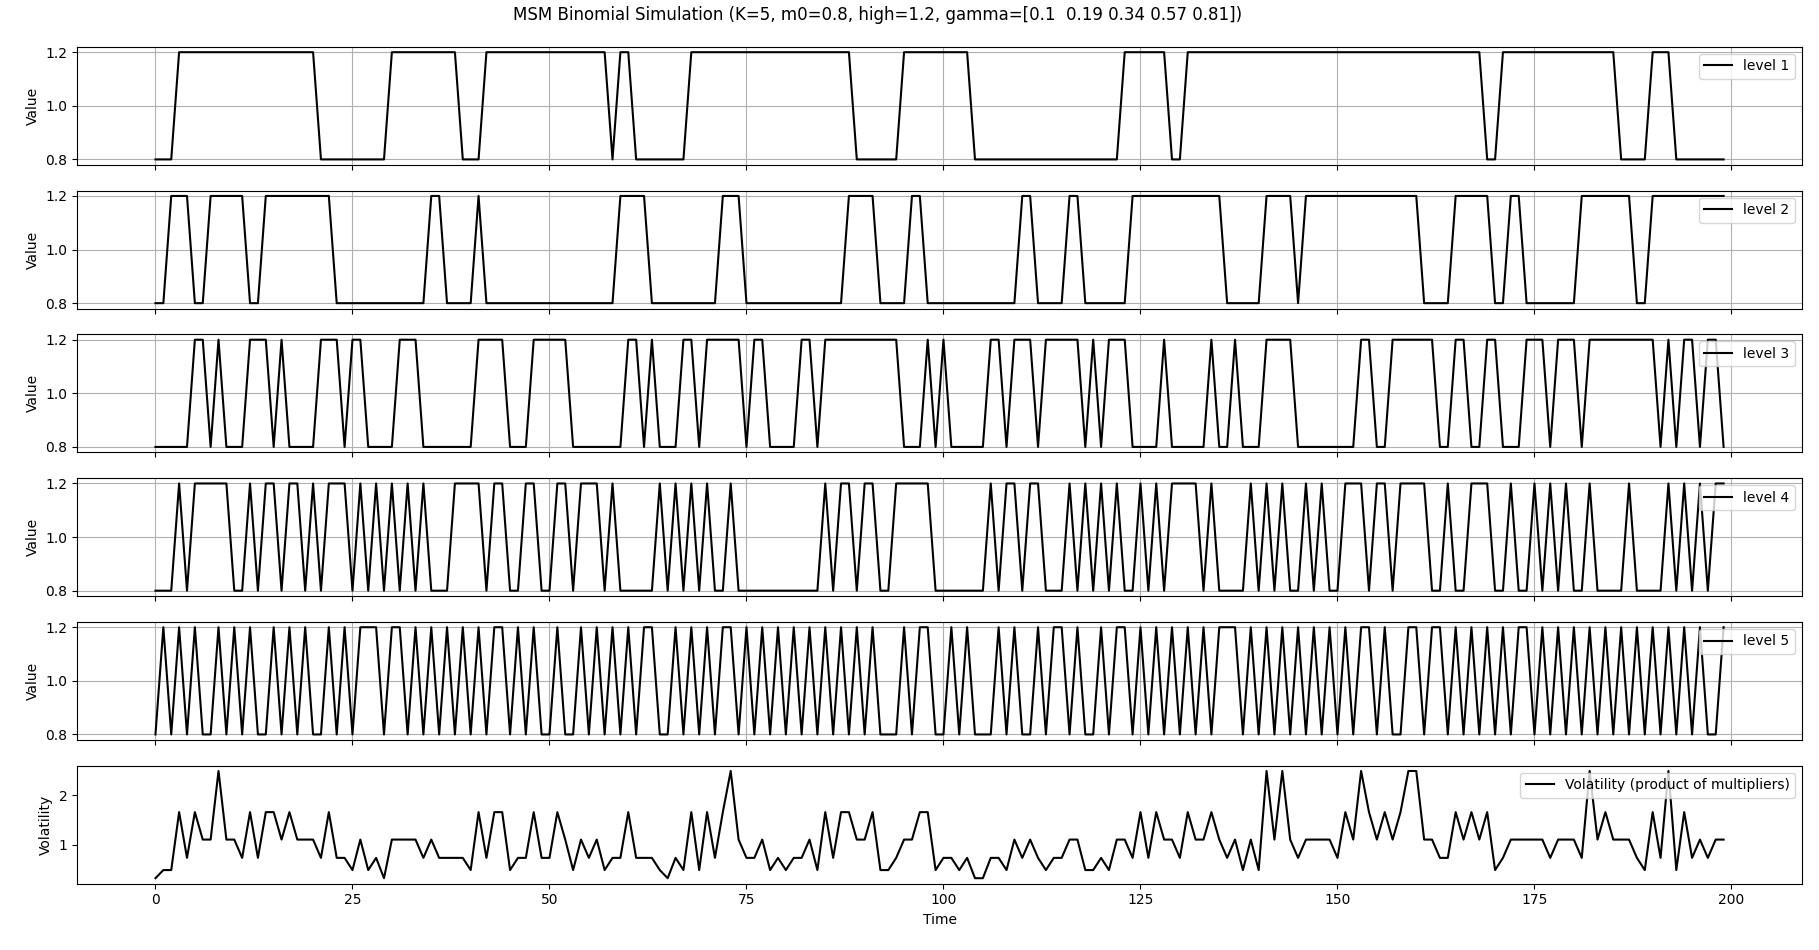
\includegraphics[width=0.8\textwidth]{img/k_analysis}
    \caption{Probability of switching at each k level in the MSM model, from top to bottom show increasing values of k.
    The simulation was performed for K=5, m0 = 0.8, 2-m0 = 1.2 and gamma [0.1, 0.19 0.34 0.57 0.81].}
    \label{fig:k_analysis}
\end{figure}

\FloatBarrier

Low-frequency multipliers $m_{t,k}$ build a fundamental block for persistent volatility.
A change in these low-level multipliers implies a strong tendency for movements in multiplied volatility.

Intermediate-frequency multipliers $m_{t,k}$ provide a smoother transition of volatility states,
effectively playing the role of a moving average in volatility. The resulting volatility may exhibit
clustering, largely due to highly correlated volatility components across different time scales.


High-frequency multipliers $m_{t,k}$ introduce additional outliers by directly affecting the
tails of the MSMF process (CalvetFisher2005). These volatility components are very short-lived and,
in extreme cases, resemble noise. As a result, it is not straightforward to capture the effect of this
component above certain thresholds of $\bar{k}$.

\subsection{Transition Dynamics and Likelihood}
Since each $M_{k,t}$ follows a two-state Markov chain, the joint process $\bigl(M_{1,t}, \dots, M_{K,t}\bigr)$ has $2^K$ states. We construct a $2^K \times 2^K$ transition matrix $\mathbf{A}$ encoding the probabilities of switching or staying in the same value at each level. The stationary distribution of $\mathbf{A}$ provides the initial state probabilities for the filtering procedure.

To estimate model parameters $(m_0,\,\gamma_1,\,b,\,\sigma)$, we maximize the log-likelihood of the observed returns. Let $\pi_t$ be the probability distribution over the $2^K$ states at time $t$. The likelihood is updated recursively via a forward filter:
\begin{enumerate}
    \item Compute the conditional density of $x_t$ given each state $s_j$,
          using $\sigma \sqrt{\prod_{k=1}^K M_{k,t}^{(j)}}$ as the volatility.
    \item Propagate $\pi_{t-1}$ through $\mathbf{A}$ and weight by the conditional densities.
    \item Normalize to obtain $\pi_t$ and accumulate the log-likelihood.
\end{enumerate}
This procedure iterates over all observations $x_1,\ldots,x_T$, yielding the maximum-likelihood estimates for the MSM parameters once the log-likelihood is maximized.

The MSM framework captures volatility clustering through a cascade of multiplicative factors, each operating on different timescales. Fast-switching levels introduce short-term fluctuations, while slow-switching levels generate persistent volatility regimes. As shown by Calvet and Fisher (2004), this hierarchical structure can replicate a wide range of stylized facts observed in financial returns, such as fat-tailed distributions and long-memory effects in volatility.





\subsection{MSM for depicting volatility}

\begin{figure}[!ht]
    \centering
    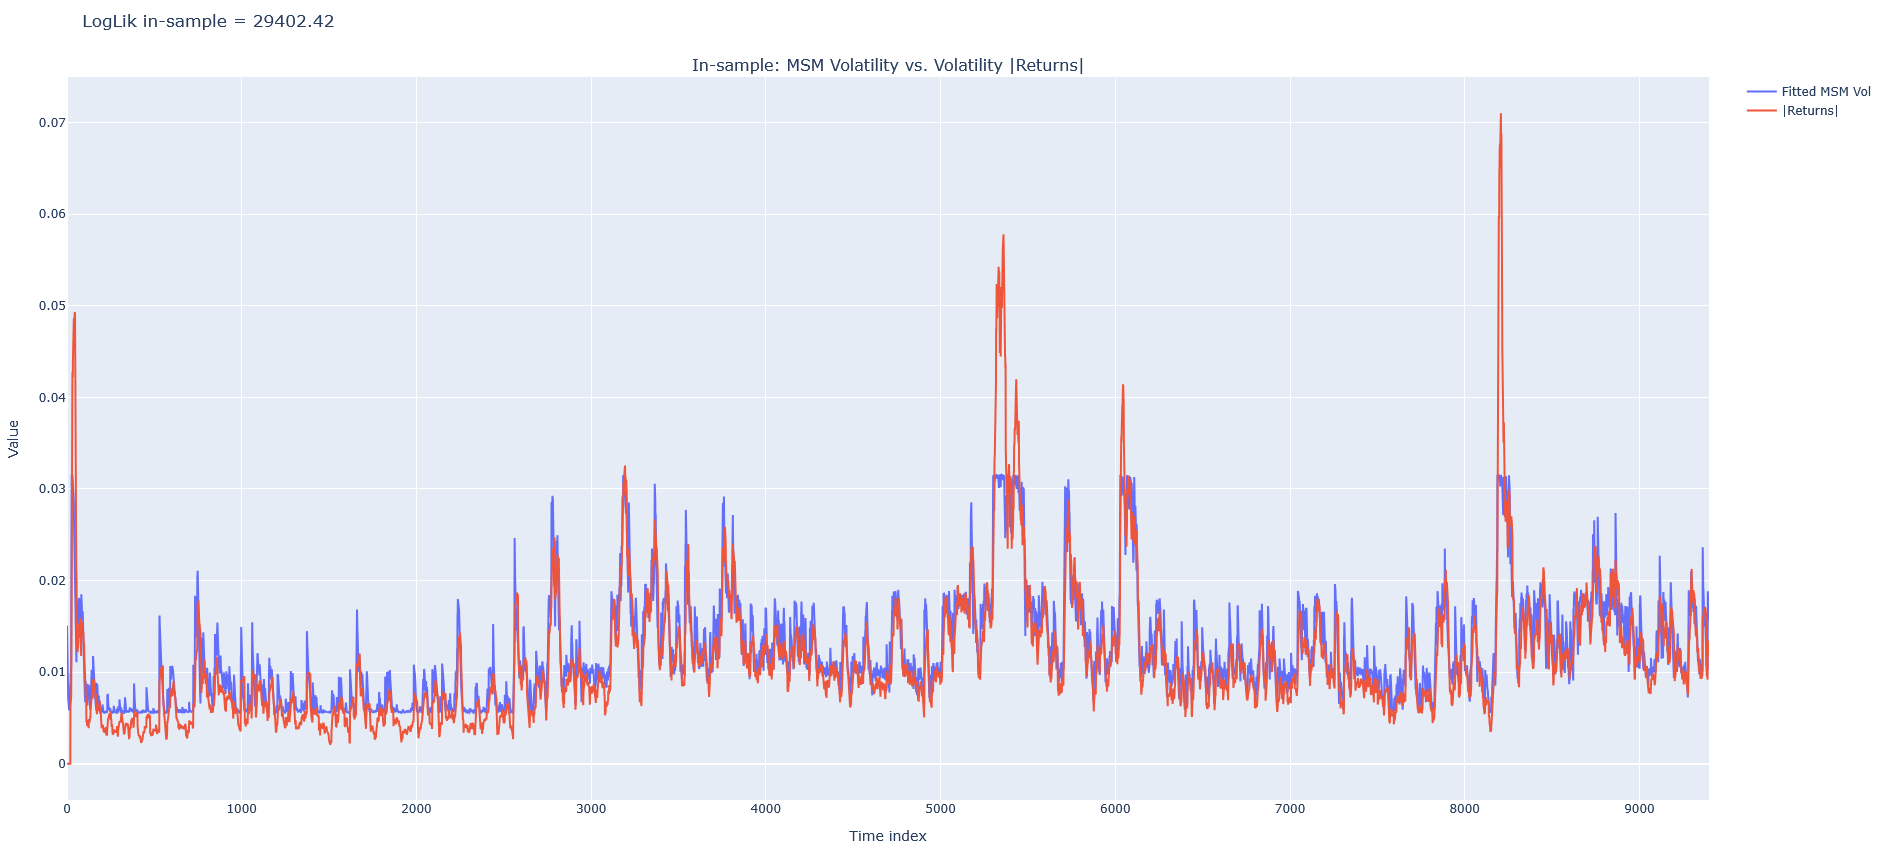
\includegraphics[width=0.8\textwidth]{img/msm_vol}
    \caption{Fitted volatility in sample and volatility of Russel 2000 returns, with MSM.}
    \label{fig:msm_fitted_vol}
\end{figure}

\FloatBarrier

Best param (m0, gamma1, sigma) = (0.46842105263157896, 0.01, 0.01663157894736842) \\

LogLik = 29402.418073294393 \\

RMSE between fitted volatility and realized volatility = 0.0032690964001980878 \\

Correlation coefficient = 0.9085561692670849 \\



\subsection{Comparison of the MSM with GARCH(1,1)}

\begin{figure}[!ht]
    \centering
    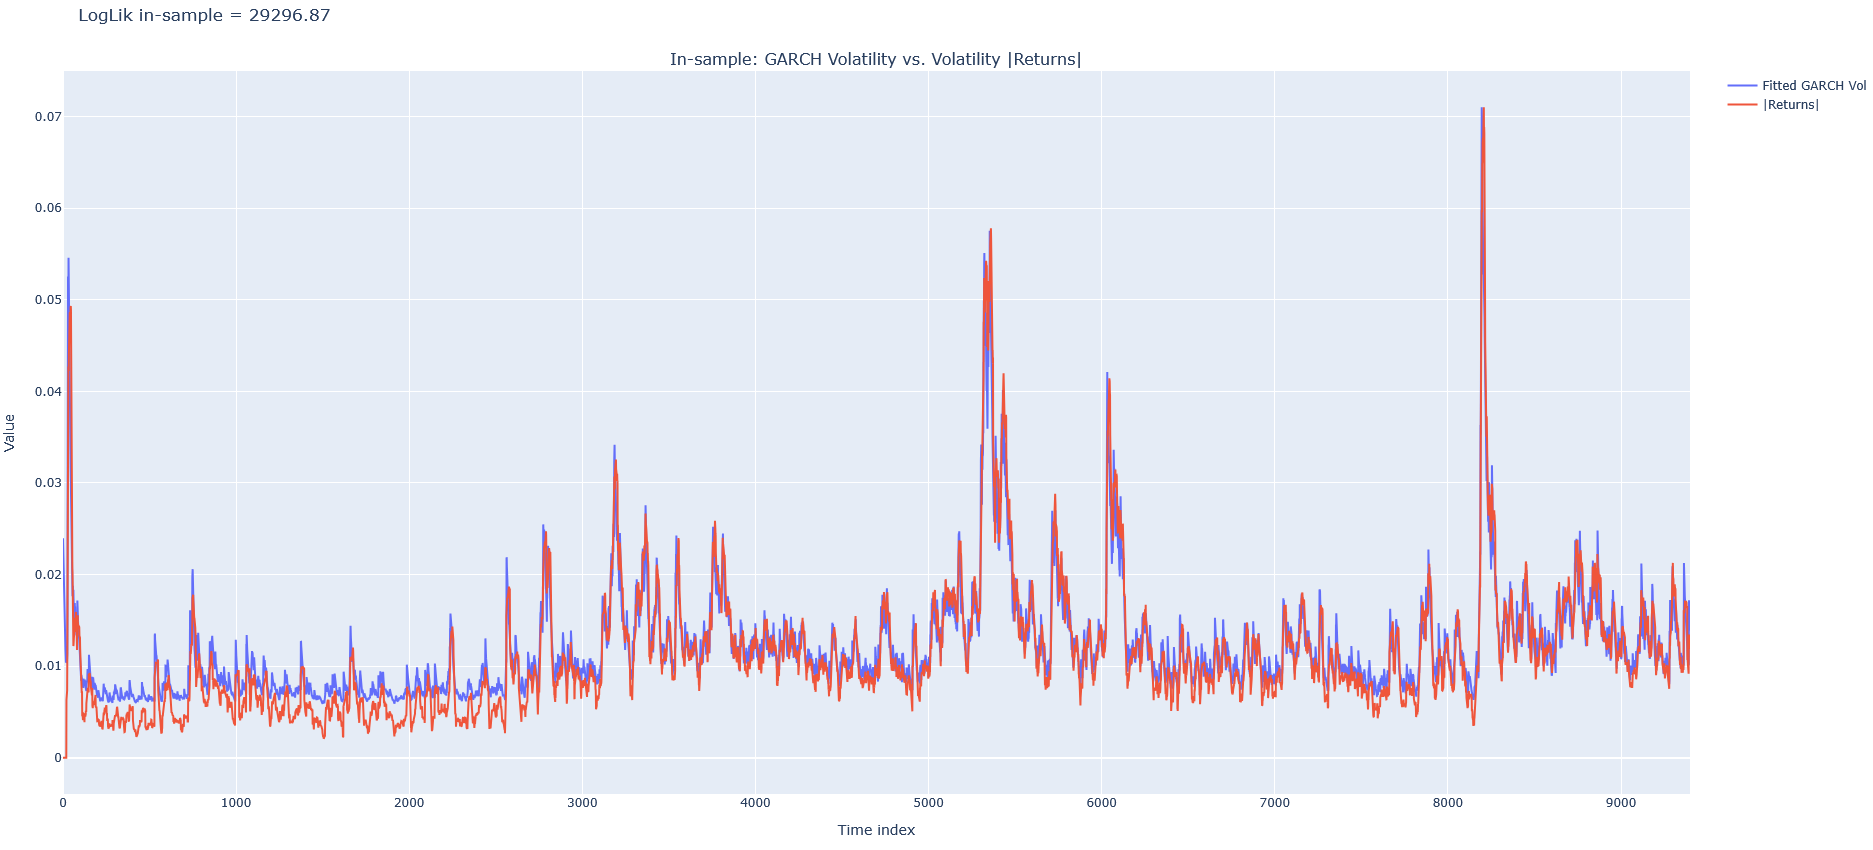
\includegraphics[width=0.8\textwidth]{img/garch_vol}
    \caption{Fitted volatility in sample and volatility of Russel 2000 returns, with garch(1,1).}
    \label{fig:garch_fitted_vol}
\end{figure}

\FloatBarrier

RMSE between GARCH volatility and realized volatility = 0.0023021519154493224 \\

Correlation coefficient GARCH = 0.9615264660690124 \\

\section{Appendix}

The critical values for the Modified R/S test are provided in the table below. These values are used to assess whether the series exhibits long memory behavior based on the Modified R/S statistic.

\begin{table}[ht!]
\centering
\begin{tabular}{|c|c|c|}
\hline
\textbf{Significance Level} & \textbf{Critical Value (Modified R/S Statistic)} \\
\hline
0.005 & 2.098\\
0.05 & 1.747\\
0.10 & 1.620\\

\hline
\end{tabular}
\caption{Critical values for the Modified R/S Statistic (Lo, 1991)}
\end{table}

\begin{table}[h!]
    \centering
    \pgfplotstabletypeset[
        col sep=comma,
        header=true,
        string type,
        every head row/.style={before row=\hline, after row=\hline},
        every last row/.style={after row=\hline},
        columns/Ticker/.style={column name=Ticker, string type},
        columns/P-Value of prices/.style={column name=P-Value of Prices, fixed, precision=3},
        columns/P-Value of log differentiated return/.style={column name=P-Value of Log Differentiated Return, fixed, precision=3}
    ] {data/adf_results.csv}
    \caption{P-values from the Augmented Dickey-Fuller (ADF) test for stationarity. The P-value of prices refers to the Augmented Dickey Fuller test (ADF) on the original series,
     while the P-value of log-differentiated returns indicates the ADF test on log-differentiated returns. The null hypothesis is non-stationarity.}
    \label{tab:adf_results}
\end{table}

\FloatBarrier


\begin{table}[ht]
    \centering
    \caption{Hurst Statistics for ticker}
    \pgfplotstableread[col sep=comma]{
Ticker, Count, Mean, Std, Min, 25, 50, 75, Max
AAPL,7299.0,1.192,0.228,0.654,1.017,1.178,1.336,1.876
JPM,7299.0,1.134,0.208,0.656,0.986,1.116,1.261,1.835
JNJ,7299.0,1.092,0.198,0.637,0.944,1.084,1.222,1.846
XOM,7299.0,1.082,0.215,0.587,0.936,1.056,1.174,1.816
WMT,7299.0,1.113,0.171,0.614,1.003,1.105,1.215,1.752
BA,7299.0,1.128,0.181,0.588,0.993,1.145,1.261,2.079
DIS,7299.0,1.184,0.238,0.633,1.008,1.159,1.362,1.979
LIN,7299.0,1.025,0.197,0.534,0.88,0.999,1.168,1.74
NEE,7299.0,1.104,0.193,0.595,0.973,1.106,1.235,1.761
SPG,7299.0,1.113,0.204,0.63,0.951,1.096,1.275,1.784
    }\datatable

    \pgfplotstabletypeset[
        every head row/.style={before row=\toprule, after row=\midrule},
        every last row/.style={after row=\bottomrule},
        columns/Ticker/.style={string type}
    ]{\datatable}
\end{table}
\FloatBarrier

\section{References}

Lo, A.W. (1991). \textit{\href{http://www.e-m-h.org/Lo\_\_91.pdf}{Long-Term Memory in Stock Market Prices}}. \\

Mignon, V. (2003). \textit{\href{https://www.persee.fr/doc/ecop_0249-4744_1998_num_132_1_5909}{Méthodes d'estimation de l'exposant de Hurst. Application aux rentabilités boursières}}, Économie \& Prévision.

Andrews, D.W.K. (1991). \textit{\href{https://www.jstor.org/stable/2938229}{Heteroskedasticity and Autocorrelation Consistent Covariance Matrix Estimation}}. \textit{Econometrica}, 59(3), 817-858.

Mandelbrot, B.B. and Wallis, J.R. (1968). "Noah, Joseph, and Operational Hydrology", \textit{Water Resources Research}, vol. 4, pp. 909--918.

Mandelbrot, B.B. (1973). "Le problème de la réalité des cycles lents et le syndrome de Joseph", \textit{Economie Appliquée}, vol. 26, pp. 349--365.

Mandelbrot, B.B. and Wallis, J.R. (1969d). "Some Long-Run Properties of Geophysical Records", \textit{Water Resources Research}, vol. 5, pp. 321--340.

Mandelbrot, B.B. and Wallis, J.R. (1969e). "Robustness of the Rescaled Range R/S in the Measurement of Noncyclic Long-Run Statistical Dependence", \textit{Water Resources Research}, vol. 5, pp. 967--988.

Mandelbrot, B.B. and Taqqu, M.S. (1979). "Robust R/S Analysis of Long-Run Serial Correlation", \textit{Bulletin of the International Statistical Institute}, vol. 48, pp. 69--104.

\end{document}
